\documentclass[14pt]{extarticle}
\usepackage{extsizes}
\usepackage[top=0.75in, bottom=0.5in, left=0.5in, right=0.5in]{geometry}
\usepackage{amsmath,amsfonts, color, booktabs, centernot, textcomp,amssymb,graphicx,verbatim,enumerate, bbm}
%\usepackage [autostyle, english = american]{csquotes}
%\usepackage [style = american]{csquotes}
%\MakeOuterQuote{"}
\usepackage{algorithm} % Boxes/formatting around algorithms
\usepackage[noend]{algpseudocode} % Algorithms
\usepackage{wrapfig}
\usepackage{fancyhdr}
\pagestyle{fancy}
\setlength\parindent{0pt}
\usepackage[linktoc=all,hidelinks]{hyperref}
%\setcounter{tocdepth}{3} % should be default
\setcounter{secnumdepth}{0}
\newcounter{problemnumber}
\def\Name{Leah Dickstein}

%\date{\today}
\lhead{\Name}
\rhead{}

\begin{document}
\title{Spring 2016}
\author{\Name \vspace{-2ex}}
\maketitle

\tableofcontents

\section{System Setup}

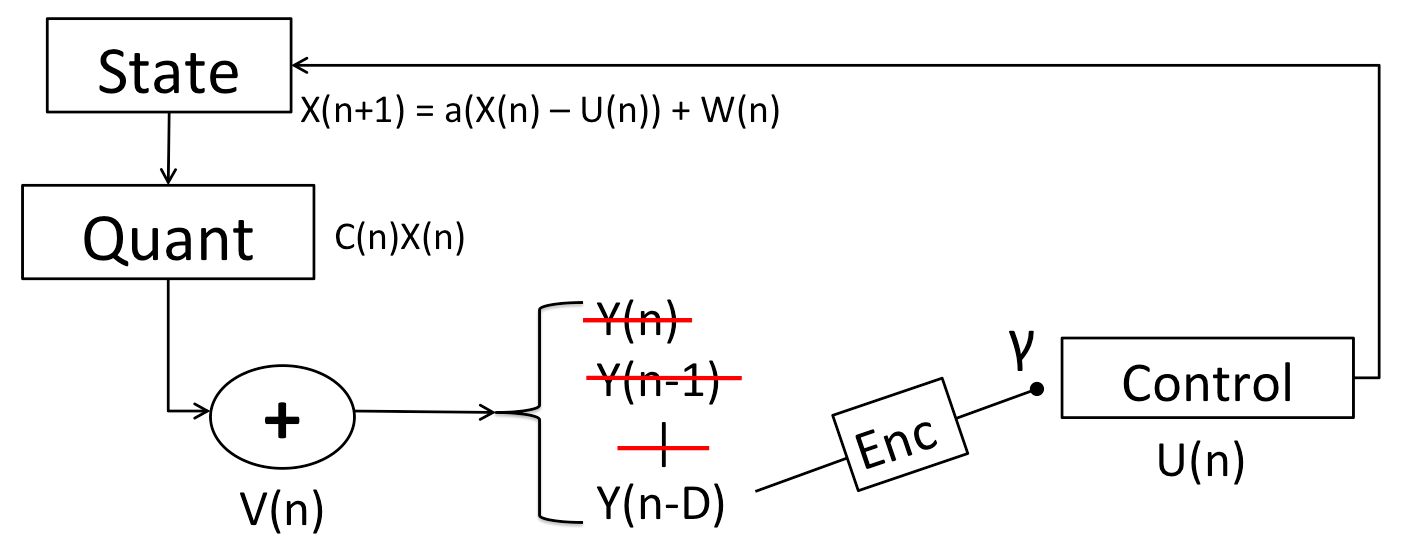
\includegraphics[width=0.5\textwidth]{sys_dynamics}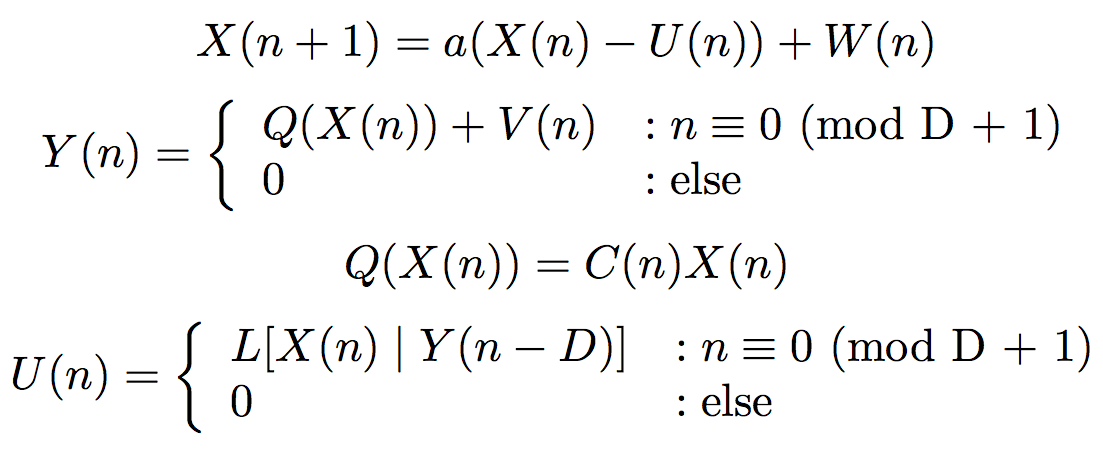
\includegraphics[width=0.5\textwidth]{sys_equations}
% 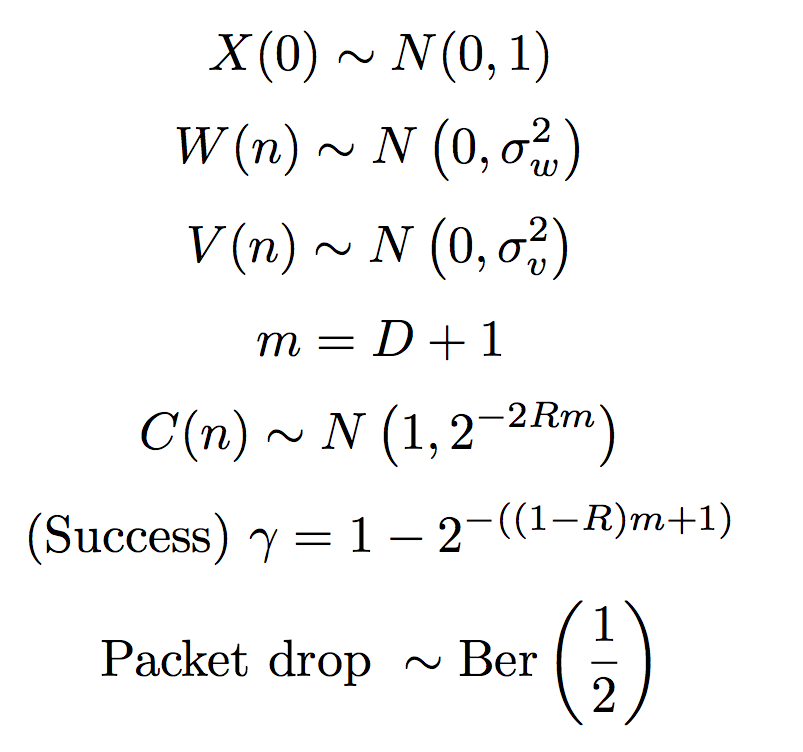
\includegraphics[width=0.35\textwidth]{sys_params}

\section{New Cost Function -- Penalize Large Control Power}

\subsection{Optimal Control -- No V(n), $\gamma = 1$, No Delay}

\[ \text{min } \mathbb{E} [ x^2(n+1) ] + \sum_{k=1}^n u^2(k) \]

\begin{math}
\text{min } \mathbb{E} [  a( x(n) - u(n) ) + w(n) )^2 ] + \sum_{k=1}^n u^2(k) \\
= \text{min } \mathbb{E} [( a( x(n) - \alpha(n) y(n) ) + w(n) )^2 ] + \sum_{k=1}^n \alpha^2(k) y^2(k) \\
= \text{min } \mathbb{E} [( a( x(n) - \alpha(n) c(n)x(n) ) + w(n) )^2 ] + \sum_{k=1}^n \alpha^2(k) c^2(k) x^2(k) \\
= \text{min } \mathbb{E} [ a^2 (1 - \alpha c(n) )^2 x^2(n) ] + \sigma_w^2 + \sum_{k=1}^n \alpha^2(k) y^2(k) \\
\frac{d}{d \alpha(n)} \mathbb{E} [ a^2 (1 - \alpha(n) c(n) )^2 x^2(n) ] + \sigma_w^2 + \sum_{k=1}^n \alpha^2(k) y^2(k) = \mathbb{E} [2a^2 (1 - \alpha(n) c(n) ) (-c(n)) x^2(n) ] + 2 \alpha(n) y^2(n)= 0 \\
-a^2 ( \mu_c \sigma_{x(n)}^2 - \alpha(n) (\mu_c^2 + \sigma_c^2 ) \sigma_{x(n)}^2 ) + \alpha(n) y^2(n) = 0 \\
\alpha(n) (a^2 (\mu_c^2 + \sigma_c^2 ) \sigma_{x(n)}^2 + y^2(n) ) = a^2 \mu_c \sigma_{x(n)}^2
\end{math}

\[ \alpha(n) = \frac{a^2 \mu_c \sigma_{x(n)}^2}{a^2 (\mu_c^2 + \sigma_c^2) \sigma_{x(n)}^2 + y^2(n)} \]

This is easy to implement, and my next step is to implement this. My worry is that this isn't a closed solution like the previous $\alpha$ calculations. As time passes, $\alpha$ will change every time a new control is implemented--which is fine, but we should note the new complication. Does this answer make sense? Should I go ahead and implement this?

\subsection{A Bound -- No V(n), $\gamma = 1$, No Delay}

\[ \alpha(n) = \frac{a^2 \mu_c \sigma_{x(n)}^2}{a^2 (\mu_c^2 + \sigma_c^2) \sigma_{x(n)}^2 + y^2(n)} \]

\begin{math}
\mathbb{E} [x^2(n+1)] \\
= \mathbb{E} [( ax(n) - a\alpha y(n) + w(n) )^2] \\
= \mathbb{E} [( ax(n) - a\alpha c(n)x(n) + w(n) )^2] \\
= \mathbb{E} [( a(1-\alpha c(n))x(n) + w(n) )^2 ] \\
a^2 (1 - 2\alpha \mu_c + \alpha^2 (\mu_c^2 + \sigma_c^2) ) < 1
\end{math}

\[ a^2 \left( 1 - \frac{2 a^2 \mu_c^2 \sigma_{x(n)}^2}{a^2 (\mu_c^2 + \sigma_c^2) \sigma_{x(n)}^2 + y^2(n)} + \frac{a^4 \mu_c^2 \sigma_{x(n)}^4 (\mu_c^2 + \sigma_c^2) }{(a^2 (\mu_c^2 + \sigma_c^2) \sigma_{x(n)}^2 + y^2(n))^2} \right) < 1 \]

As this is similar to original cost function with V(n), I don't believe this is easily simplifiable. This should just be calculated in code/implementation.

\section{Original Cost Function: Minimize Mean Square State}

\subsection{Optimal Control -- No V(n), $\gamma = 1$, Delay}

\[ \text{min } \mathbb{E} [x^2(n+1) ] \]

\begin{math}
\text{min } \mathbb{E} [( a (x(n) - \alpha y(n-D) ) + w(n) )^2 ] \\
= \text{min } \mathbb{E} [( a (x(n) - \alpha c(n-D)x(n-D) ) + w(n) )^2] \\
= \text{min } \mathbb{E} [( a (a^Dx(n-D) + \sum_{i=1}^D a^{i-1} w(n-i) - \alpha c(n-D)x(n-D) ) + w(n) )^2] \\
= \text{min } \mathbb{E} [( a(a^D - \alpha c(n-D) x(n-D) + \sum_{i=0}^D a^i w(n-i) )^2 ] \\
\frac{d}{d \alpha} \downarrow = \mathbb{E} [2a^2 (a^D - \alpha c(n-D) ) x^2(n-D) (-c(n-D)) ] = 0 \\
\mathbb{E}[c(n-D) (a^D - \alpha c(n-D)) x^2(n-D) ] = 0 \\
a^D \mu_c \sigma^2_{x(n-D)} = \alpha (\mu_c^2 + \sigma_c^2) \sigma^2_{x(n-D)}
\end{math}

\[ \alpha = \frac{a^D \mu_c}{\mu_c^2 + \sigma_c^2} \]

The addition of delay simply means our control has to project into the future (by a scaling factor) for when it will be applied.

\subsection{A Bound -- No V(n), $\gamma = 1$, Delay}

\[ \alpha = \frac{a^D \mu_c}{\mu_c^2 + \sigma_c^2} \]

\begin{math}
\mathbb{E} [( a(x(n) - \alpha y(n-D)) + w(n) )^2] \\
= \mathbb{E} [( ax(n) - a\alpha y(n-D) + w(n) )^2] \\
= \mathbb{E} [( a^{D+1}x(n-D) - a\alpha y(n-D) + \sum_{i=0}^D a^i w(n-i) )^2 ] \\
= \mathbb{E} [( a^{D+1}x(n-D) -a\alpha c(n-D)x(n-D) + \sum_{i=0}^D a^i w(n-i) )^2] \\
= \mathbb{E} [(a^{D+1} - a\alpha c(n-D))^2 x^2(n-D) ] + \mathbb{E} [\sum_{i=0}^D a^{2i} w^2(n-i) ] \\
a^{2(D+1)} - 2a^{D+2} \alpha \mu_c + a^2 \alpha^2 (\mu_c^2 + \sigma_c^2 ) < 1 \\
a^{2(D+1)} - \frac{2a^{2(D+1)} \mu_c^2}{\mu_c^2 + \sigma_c^2} + \frac{a^{2(D+1)} \mu_c^2}{\mu_c^2 + \sigma_c^2} < 1 \\
a^{2(D+1)} - \frac{a^{2(D+1)} \mu_c^2}{\mu_c^2 + \sigma_c^2} < 1 \; \rightarrow \;  a^{2(D+1)} \left( 1 - \frac{\mu_c^2}{\mu_c^2 + \sigma_c^2} \right) < 1 \; \rightarrow \; a^{2(D+1)} < \frac{\mu_c^2 + \sigma_c^2}{\sigma_c^2}
\end{math}

\[  a^{2(D+1)} < \frac{\mu_c^2 + \sigma_c^2}{\sigma_c^2} \quad \quad a < \left( \frac{\mu_c^2 + \sigma_c^2}{\sigma_c^2} \right)^{\frac{1}{2(D+1)}} \]

\subsection{Optimal Control -- No V(n), $\gamma = 1$, No Delay}

\[ \text{min } \mathbb{E} [x^2(n+1) ] \]
\[ u(n) = \alpha y(n) = \alpha c(n) x(n) \]

\begin{math}
\text{min } \mathbb{E} [( a( x(n) - u(n) ) + w(n) )^2 ] \\
= \text{min } \mathbb{E} [( a( x(n) - \alpha y(n) ) + w(n) )^2 ] \\
= \text{min } \mathbb{E} [( a( x(n) - \alpha c(n)x(n) ) + w(n) )^2 ] \\
= \text{min } \mathbb{E} [ a^2 (1 - \alpha c(n) )^2 x^2(n) ] + \sigma_w^2 \\
\frac{d}{d \alpha} \mathbb{E} [ a^2 (1 - \alpha c(n) )^2 x^2(n) ] + \sigma_w^2 = \mathbb{E} [2a^2 (1 - \alpha c(n) ) (-c(n)) x^2(n) ] = 0 \\
\mathbb{E} [c(n) x^2(n) - \alpha c^2(n) x^2(n) ] = 0 \\
\mu_c \sigma_{x(n)}^2 = \alpha (\mu_c^2 + \sigma_c^2 ) \sigma_{x(n)}^2
\end{math}

\[ \alpha = \frac{\mu_c}{\mu_c^2 + \sigma_c^2} \]

These are the results we expect, from Gireeja's Noncoherence Paper.

\subsection{Optimal Control -- V(n), $\gamma = 1$, Delay}

\[ \text{min } \mathbb{E} [x^2(n+1) ] \]

\begin{math}
\text{min } \mathbb{E} [( ax(n) - a\alpha y(n-D) + w(n) )^2] \\
= \text{min } \mathbb{E} [( a^{D+1}x(n-D) + \sum_{i=0}^D a^i w(n-i) -a\alpha y(n-D) )^2 ] \\
= \text{min } \mathbb{E} [( a^{D+1}x(n-D) -a\alpha c(n-D)x(n-D) -a\alpha v(n-D) + \sum_{i=0}^D a^i w(n-i) )^2] \\
\frac{d}{d\alpha} \downarrow = \mathbb{E} [-2a^{D+2} c(n-D) x^2(n-D) + 2\alpha a^2 c^2(n-D) x^2(n-D) + 2a^2 \alpha v^2(n-D) ] = 0 \\
-a^{D+2} \mu_c \sigma_{x(n-D)}^2 + \alpha a^2 (\mu_c^2 + \sigma_c^2) \sigma^2_{x(n-D)} + \alpha a^2 \sigma_v^2 = 0 \\
\alpha ( (\mu_c^2 + \sigma_c^2) \sigma_{x(n-D)}^2 + \sigma_v^2 ) = a^D \mu_c \sigma^2_{x(n-D)}
\end{math}

\[ \alpha(n) = \frac{a^D \mu_c \sigma_{x(n-D)}^2}{(\mu_c^2 + \sigma_c^2) \sigma_{x(n-D)}^2 + \sigma_v^2} \]

\subsection{A Bound -- V(n), $\gamma = 1$, Delay}

\[ \alpha(n) = \frac{a^D \mu_c \sigma_{x(n-D)}^2}{(\mu_c^2 + \sigma_c^2) \sigma_{x(n-D)}^2 + \sigma_v^2} \]

\begin{math}
\mathbb{E} [a^{2(D+1)}x^2(n-D) -2a^{D+2}\alpha(n) c(n-D) x^2(n-D) + a^2 \alpha^2(n) c^2(n-D) x^2(n-D) ] \\
a^{2(D+1)} - 2a^{D+2} \alpha(n) \mu_c + a^2 \alpha^2(n) (\mu_c^2 + \sigma_c^2) < 1 \\
a^{2(D+1)} - \frac{2a^{2(D+1)} \mu_c \sigma^2_{x(n-D)}}{(\mu_c^2 + \sigma_c^2) \sigma_{x(n-D)}^2 + \sigma_v^2 } + \frac{a^{2(D+1)} \mu_c^2 \sigma^4_{x(n-D)} (\mu_c^2 + \sigma_c^2)}{((\mu_c^2 + \sigma_c^2) \sigma_{x(n-D)}^2 + \sigma_v^2)^2} < 1
\end{math}

\[ a^{2(D+1)} \left( 1 - \frac{2\mu_c^2 \sigma^2_{x(n-D)}}{(\mu_c^2+\sigma_c^2) \sigma^2_{x(n-D)} + \sigma_v^2} + \frac{\mu_c^2 \sigma^4_{x(n-D)} (\mu_c^2 + \sigma_c^2)}{((\mu_c^2 + \sigma_c^2) \sigma^2_{x(n-D)} + \sigma_v^2 )^2} \right) < 1 \]

This is really ugly. I started looking into simplifying it, but I don't think it can be simplified further. It would be best to directly calculate everything out in implementation/code. 

\subsection{Optimal Control -- V(n) $\gamma = 1$, No Delay}

\[ \text{min } \mathbb{E} [x^2(n+1) ] \]

\begin{math}
\text{min } \mathbb{E} [ ( a(1-\alpha c(n) ) x(n) - a\alpha v(n) + w(n) )^2 ] \\
= \text{min } \mathbb{E}[ a^2 (1-\alpha c(n) )^2 x^2(n) + \mathbb{E} [a^2 \alpha^2 v^2(n) ] + \sigma_w^2 \\
\frac{d}{d \alpha}  \mathbb{E}[ a^2 (1-\alpha c(n) )^2 x^2(n) + \mathbb{E} [a^2 \alpha^2 v^2(n) ] + \sigma_w^2 = \mathbb{E}[ -2a^2 (1-\alpha c(n)) c(n) x^2(n) ] + 2 a^2 \alpha \sigma_v^2 = 0\\
= -\mu_c \sigma_{x(n)}^2 + \alpha (\mu_c^2 + \sigma_c^2 ) \sigma_{x(n)}^2 + \alpha \sigma_v^2 = 0
\end{math}

\[ \alpha(n) = \frac{\mu_c \sigma_{x(n)}^2}{(\mu_c^2 + \sigma_c^2) \sigma_{x(n)}^2 + \sigma_v^2} \]

These are the results we expect from the LLSE theorem: $\alpha = \frac{cov(X, Y)}{var(Y)} = \frac{\mathbb{E}[XY]}{\mathbb{E}[Y^2]} \leftarrow \text{assuming } \mathbb{E}[X] = \mathbb{E}[Y] = 0 $

\subsection{With No Delay, Memoryless Control is Optimal - Full Noise}

Setup:
\begin{align*}
x(n+1) & = a(x(n) - u(n)) \\
y(n) & = c(n)x(n) + v(n) \\
u(n) & = \alpha(n)y(n) + \beta(n)y(n-1)
\end{align*}

\begin{math}
\text{min } \mathbb{E}[x^2(n+1)] = \text{min } a^2 \; \mathbb{E}[( x(n) - u(n) )^2] \\
= \text{min } a^2 \mathbb{E} [ ( x(n) - \alpha(n)y(n) - \beta(n)y(n-1) )^2] \\
\frac{d}{d \beta(n)} \; a^2 \; \mathbb{E} [ ( x(n) - \alpha(n)y(n) - \beta(n)y(n-1) )^2] = \\
a^2 \; 2 \; \mathbb{E} [ (-y(n-1)) ( x(n) - \alpha(n)y(n) - \beta(n)y(n-1) ) ] = 0 \\
\mathbb{E} [ x(n)y(n-1) - \alpha(n)y(n)y(n-1) - \beta(n)y^2(n-1) ] = 0 \\
\beta(n) \mathbb{E} [y^2(n-1)] = \mathbb{E}[ x(n)y(n-1) - \alpha(n) (c(n)x(n) + v(n)) y(n-1) ] \\
\beta(n) \mathbb{E} [ y^2(n-1) ] = \mathbb{E} [ (1-\alpha(n)c(n)) x(n) y(n-1) ] \\
\beta(n) \mathbb{E} [ y^2(n-1) ] = \mathbb{E} [1-\alpha(n)c(n)] \; \mathbb{E} [x(n)y(n-1)] \\
\end{math}

From here, we can see that $\mathbb{E} [x(n)y(n-1)] = 0$ or is uncorrelated. This is because when there is no delay, the content of the previous observation has already been killed by the current timestep, so the current timestep state is uncorrelated with all previous observations. In other words, there is no need for memory because from the perspective of the controller, it has succeeded in bringing the state to 0. I will now prove $\mathbb{E} [x(n)y(n-1)] = 0$, just to be sure. \\

\begin{math}
\mathbb{E}[x(n)y(n-1)] = \mathbb{E}[ax(n-1)y(n-1) - au(n-1)y(n-1)] \\
= a \mathbb{E} [x(n-1)y(n-1) - \alpha(n-1)y^2(n-1) - \beta(n-1)y(n-2)y(n-1) ] \\
= a \left( \mathbb{E} [x(n-1)y(n-1)] - \alpha(n-1) \mathbb{E}[y^2(n-1)] - \beta(n-1) \mathbb{E} [y(n-2)y(n-1)] \right) \\
\end{math}

Assume $\beta(n-1) = 0$ and $\alpha(n-1) = \frac{\mathbb{E}[x(n-1)y(n-1)]}{\mathbb{E}[y^2(n-1)]}$. These are valid assumptions based on how the control is initialized. Then:

\[ \mathbb{E}[x(n)y(n-1)] = a \left( \mathbb{E} [x(n-1)y(n-1)] - \frac{\mathbb{E}[x(n-1)y(n-1)]}{\mathbb{E}[y^2(n-1)]} \; \mathbb{E}[y^2(n-1)] - 0 \right) = 0 \]

Therefore, $\beta(n) \; \mathbb{E}[y^2(n-1)] = \mathbb{E} [1-\alpha(n)c(n)] \cdot 0 = 0 \implies \forall n \; \beta(n) = 0$.\\

Some notes:
\begin{enumerate}[1:]
\item Cost function, replace x(n+1) with definition
\item Replace u(n)
%\item Take derivative with respect to $\beta(n)$, wish to prove $\forall n \; \beta(n) = 0$
\item[6:] v(n) is independent of other variables and 0-mean, so it goes away
\item[7:] $(1-\alpha(n)c(n))$ is independent of $x(n)y(n-1)$. We assume $\alpha(n)$ is a constant $\alpha(n) \in \mathbb{R}$, thus it is independent of all RVs. $x(n)$ is dependent on $c(n-1)$ but independent of $c(n)$. In addition, $c(n)$ is independent of previous timesteps, including $y(n-1)$.
\end{enumerate}

Also note, this can be modeled as an HMM, in which case the memoryless property makes sense. The state is all innovation.\\

It is interesting to note that in the Gaussian case, the LLSE is the MMSE and is therefore the optimal control. In this case, multiplicative noise means the observation is no longer Gaussian, yet the memoryless LLSE remains optimal. This makes sense--there is no reason multiplicative noise would change anything, since control means the state is killed at each timestep. With delay, this is no longer necessarily true--memory will become important.

\section{1-Memory Control}

\[ u(n) = \alpha(n) \: y(n) + \beta(n) \: y(n-1) \]
\[ \text{min } \mathbb{E}[x^2(n+1)] = \mathbb{E}[a^2 \left( x(n) - u(n) \right)^2 ] = \mathbb{E}[a^2 \left( x(n) - \alpha(n)y(n) - \beta(n)y(n-1) \right)^2 ] \]
\[ \alpha(n) = \frac{\mathbb{E}[x(n)y(n)] \; \mathbb{E}[y^2(n-1)] - \mathbb{E}[y(n)y(n-1)] \; \mathbb{E} [x(n)y(n-1)]}{\mathbb{E}[y^2(n)] \; \mathbb{E} [y^2(n-1)] - \mathbb{E}[y(n)y(n-1)] \; \mathbb{E} [y(n)y(n-1)]} \]
\[ \beta(n) = \frac{ \mathbb{E}[x(n)y(n-1)] - \alpha(n) \mathbb{E}[y(n)y(n-1)] }{ \mathbb{E}[y^2(n-1)] } \]

Derivation: \\
\begin{math}
\frac{d}{d \, \alpha(n)} \mathbb{E}[x^2(n+1)] = \mathbb{E}[a^2 \, 2 (x(n) - \alpha(n) y(n) - \beta(n)y(n-1) ) (-y(n)) ] = 0 \\
\mathbb{E}[y(n) (x(n) - \alpha(n) y(n) - \beta(n)y(n-1) ) ] = 0 \\
\alpha(n) \mathbb{E}[y^2(n)] = \mathbb{E}[x(n)y(n)] - \beta(n) \mathbb{E} [y(n)y(n-1)] \\
\frac{d}{d \, \beta(n)} \mathbb{E} [x^2(n+1)] = \mathbb{E}[y(n-1)(x(n) - \alpha(n) y(n) - \beta(n)y(n-1) )] = 0\\
\end{math}

We can then write two linear equations (with two variables):
\[ \alpha(n) \: \mathbb{E} [y^2(n)] = \mathbb{E}[x(n)y(n)] - \beta(n) \:  \mathbb{E} [y(n)y(n-1)] \]
\[ \beta(n) \: \mathbb{E} [y^2(n-1)] = \mathbb{E}[x(n)y(n-1)] - \alpha(n) \: \mathbb{E} [y(n)y(n-1)] \]

Solve for $\alpha(n)$:\\
\begin{math}
\alpha(n) \mathbb{E} [y^2(n)] = \mathbb{E}[x(n)y(n)] - \frac{\mathbb{E}[y(n)y(n-1)]}{\mathbb{E}[y^2(n-1)]} \left( \mathbb{E}[x(n)y(n-1)] - \alpha(n) \mathbb{E}[y(n)y(n-1)] \right) \\
\alpha(n) \left( \mathbb{E}[y^2(n)] - \frac{\mathbb{E}[y(n)y(n-1)]^2}{\mathbb{E}[y^2(n)]} \right) = \mathbb{E}[x(n)y(n)] - \frac{\mathbb{E}[y(n)y(n-1)] \mathbb{E}[x(n)y(n-1)]}{\mathbb{E}[y^2(n-1)]} \\
\alpha(n) \left( \mathbb{E}[y^2(n)] \mathbb{E}[y^2(n-1)] - \mathbb{E}[y(n)y(n-1)]^2 \right) = \mathbb{E}[x(n)y(n)] \mathbb{E} [y^2(n-1)] - \mathbb{E}[y(n)y(n-1)] \mathbb{E}[x(n)y(n-1)]\\
\end{math}

Note that if delay = 0, this simplifies to the case above (where $\forall n \; \beta(n) = 0$ and memoryless control is optimal.)

\subsection{Delay = 1 (Mod 2)}

Boolean table with 8 entries:\\

%\begin{table}[]
{\centering
%\label{my-label}
\begin{tabular}{cccc}
State Noise & Multiplicative Noise & Additive Noise & Subsection Number \\ \hline
0           & 0                    & 0              & 1                 \\
0           & 0                    & 1              & 2                 \\
0           & 1                    & 0              & 3                 \\
0           & 1                    & 1              & 4                 \\
1           & 0                    & 0              & 5                 \\
1           & 0                    & 1              & 6                 \\
1           & 1                    & 0              & 7                 \\
1           & 1                    & 1              & 8                
\end{tabular}}
%\end{table}

\setcounter{secnumdepth}{3}
\subsubsection{No Noise}
Setup: \\
\begin{math}
x(n+1) = a \, x(n) \\
y(n) = x(n) \\
\end{math}

Infinite solutions: $\forall \, \alpha(n), \; \beta(n) = a \, (1 - \alpha(n))$. 
\[ \mathbb{E}[x(n) \, | \, y(n), y(n-1) ] = \alpha(n) y(n) + \beta(n) y(n-1) = \alpha(n) x(n)  + \beta(n) x(n-1) \]
\[ \hat{x}(n) = \alpha(n) \, x(n) + a(1-\alpha(n)) \, x(n-1) = \alpha(n) \, x(n) + (1-\alpha(n)) \, x(n) = x(n) \]

\subsubsection{Additive Noise only}

\subsubsection{Multiplicative Noise only}
Setup: \\
\begin{math}
x(n+1) = a \, x(n) \\
y(n) = c(n) \, x(n) \\
\end{math}

\[ \forall \, n, \quad \quad \alpha(n) = \frac{\mu_c}{2\mu_c^2 + \sigma_c^2} \quad \quad \beta(n) = \frac{a\mu_c}{2\mu_c^2 + \sigma_c^2} \]
\[ \mathbb{E}[x(n) \, | \, y(n), y(n-1)] = \frac{ \mu_c c(n) x(n) + a \mu_c c(n-1) x(n-1) }{2\mu_c^2 + \sigma_c^2} \]
\[ = \frac{\mu_c c(n) x(n) + \mu_c c(n-1) x(n)}{2\mu_c^2 + \sigma_c^2} = \frac{\mu_c \, x(n) \, ( c(n) + c(n-1))}{2\, \mu_c^2 + \sigma_c^2} \]

Unit tests:
\[ \mu_c = 1, \; \sigma_c^2 = 0 \implies \hat{x}(n) = \frac{\mu_c \, x(n) \, ( c(n) + c(n-1))}{2\, \mu_c^2 + \sigma_c^2} = x(n) \] 

\textcolor{blue}{\textbf{Note}: I have more of these calculated, but need to TeX them up!!}

\setcounter{secnumdepth}{0}

\section{Memory Control}

\subsection{Lemma: After Control is Applied, State is Uncorrelated with Previous Observations}

\textbf{Note}: I assume the optimal control is the optimal estimate given observations. I'm honestly not sure if that's a safe assumption to make, but I'm going to proceed anyway. If necessary, I'll try to prove that assumption in a separate lemma. \\

First, note the Delay = 0 case: \\
\begin{math}
x(n+1) = a(x(n) - u(n)) \\
u(n) = \mathbb{E}[x(n) \, | \, Y^n] = \mathbb{E}[x(n) \, | \, y(n)] \\
\end{math}

We have previously shown that the optimal control when delay=0 is memoryless.\\

\begin{math}
\mathbb{E}[x(n+1)y(n)] = \mathbb{E}[a(x(n)y(n) - u(n)y(n))] = a \, \mathbb{E}[x(n) \, y(n) - \mathbb{E}[x(n) \, | \, y(n)] \, y(n)] \\\\
\mathbb{E}[x(n) \, y(n)] \doteq \int \int x(n) \, y(n) \, f(x(n), y(n)) \, dx(n) \, dy(n) \\
\mathbb{E}[\mathbb{E}[x(n) \, | \, y(n)] \, y(n)] = \int \int x(n) \, f(x(n) \, | \, y(n)) \, dx(n) \, y(n) \, f(y(n)) \, dy(n)\\
= \int \int x(n) \, f(x(n), y(n)) \, dx(n) \, dy(n) \\
\therefore \mathbb{E}[u(n) \, y(n)] = \mathbb{E}[x(n) \, y(n)] \\
\therefore \mathbb{E}[x(n+1) \, y(n)] = a \cdot 0 = 0\\
\end{math}

Now, note the Delay = 1 case: \\
\begin{math}
x(n+1) = a(x(n) - u(n)) \\
u(n) = \mathbb{E}[x(n) \, | \, Y^n] = \mathbb{E}[x(n) \, | \, y(n), y(n-1)] \\
\end{math}

I could keep it as $Y^n$, but I simplify to $y(n), y(n-1)$ for clarity. By the end of this lemma, you will see why this simplification is ok. \\

\begin{math}
\mathbb{E}[x(n+1) \, y(n)] = \mathbb{E}[a \, (x(n)-u(n)) \, y(n)] = a \,  \mathbb{E}[x(n)y(n) - u(n)y(n)] \\
\mathbb{E}[x(n) \, y(n)] \doteq \int \int x(n) \, y(n) \, f(x(n), y(n)) \, dx(n) \, dy(n) \\
\mathbb{E}[u(n)y(n)] = \mathbb{E}[\mathbb{E}[x(n) | y(n), y(n-1)] \, y(n)] \\
= \int \int x(n) \, f(x(n) \, | \, y(n), y(n-1)) \, dx(n) \, y(n) \, f(y(n)) \, dy(n) \\
= \int \int x(n) \, f(x(n) \, | \, y(n), y(n-1)) \, dx(n) \, y(n) \, \int f(y(n), y(n-1)) \, dy(n-1) \, dy(n) \\
\end{math}

Now you see why previous timesteps are irrelevant. We will simply integrate over them (like reverse finding a marginal distribution.)

\begin{math}
= \int \int \int x(n) \, y(n) \, f(x(n), y(n), y(n-1)) \, dx(n) \, dy(n-1) \, dy(n) \\
= \int \int x(n) \, y(n) \, f(x(n), y(n)) \, dx(n) \, dy(n) \\
\therefore \mathbb{E}[u(n) \, y(n)] = \mathbb{E}[x(n) \, y(n)] \\
\therefore \mathbb{E}[x(n+1) \, y(n)] = 0 \\
\end{math}

Now we generalize for any delay D. I will use the same trick of turning $f(y(n))$ into an integral in $n-1$ dimensions. \\

\begin{math}
u(n) = \mathbb{E}[x(n) \, | \, Y^n ] \quad \quad Y^n \doteq y(n) \dots y(1) \\
\mathbb{E}[u(n) \, y(n)] = \mathbb{E}[ \mathbb{E}[x(n) \, | \, Y^n ] \, y(n) ] \\
= \int \int x(n) \, f(x(n) \, | \, Y^n) \, dx(n) \, y(n) \, f(y(n)) \, dy(n) \\
= \int \int x(n) \, f(x(n) \, | \, Y^n) \, dx(n) \, y(n) \, \int \cdots \int_\mathbb{R} f(Y^n) \, dy(n) \cdots dy(1) \\
= \int \int \int \cdots \int_\mathbb{R} x(n) \, y(n) \, f(x(n), y(n) \dots y(1)) \, dx(n) \, dy(n) \cdots dy(1)  \\
= \int \int x(n) \, y(n) \, f(x(n), y(n)) \, dx(n) \, dy(n) \\
\therefore \mathbb{E}[u(n) \, y(n)] = \mathbb{E}[x(n) \, y(n)] \\
\therefore \mathbb{E}[x(n+1) \, y(n)] = 0\\
\end{math}

Note that any linear function of x(n+1), such as y(n+1) or x(n+2), will also be uncorrelated with $Y^n$.\\

With this lemma proven, I can now prove that the maximum memory needed for D delay is D timesteps (then the control will be applied and observations will become uncorrelated.) I will do that either later tonight or tomorrow! I have a sketch for the delay = 1 case using $u(n) = \alpha(n) \, y(n) + \beta(n) \, y(n-1) + \gamma(n) \, y(n-2)$ but need to generalize.

\subsection{Calculating Optimal Memory-Based Control w/ Linear Algebra}

Suppose $u(n) = \sum_{i=0}^{n-1} \alpha_i(n) \, y(n-i)$.
\[ \forall \, k \in [0, n-1], \frac{d}{d\alpha_k(n)} \mathbb{E}[x^2(n+1)] = \mathbb{E} \left[ y(n-k) \, \left( x(n) - \sum_{i=0}^{n-1} \alpha_i(n) \, y(n-i) \right) \right] = 0 \]

We can set this up in matrix form, $Ax = b$, where A is $n \times n$ and x, b are $n \times 1$:

\begin{small}
\[ \begin{bmatrix}
\mathbb{E}[y(n) \, y(n)] & \mathbb{E}[y(n) \, y(n-1)] & \cdots & \mathbb{E}[y(n) \, y(1)] \\
\mathbb{E}[y(n-1) \, y(n)] & \mathbb{E}[y(n-1) \, y(n-1)] & \cdots & \mathbb{E}[y(n-1) \, y(1)] \\ 
\vdots & \vdots & \ddots & \vdots \\
\mathbb{E}[y(1) \, y(n)] & \mathbb{E}[y(1) \, y(n-1)] & \cdots & \mathbb{E}[y(1) \, y(1)]
\end{bmatrix}
\begin{bmatrix}
\alpha_0(n) \\ \alpha_1(n) \\ \vdots \\ \alpha_{n-1}(n) \end{bmatrix} = \begin{bmatrix}
\mathbb{E}[x(n) \, y(n)] \\ \mathbb{E}[x(n) \, y(n-1)] \\ \vdots \\ \mathbb{E}[x(n) \, y(1)]
\end{bmatrix} \]
\end{small}

From the previous lemma, we can zero out a lot of values and the matrix remains with a diagonal block structure.

\begin{scriptsize}
\[
\begin{bmatrix}

\begin{bmatrix}
\mathbb{E}[y(n) \, y(n)] & \cdots & \mathbb{E}[y(n) \, y(n-D)] \\ 
\vdots & \ddots & \vdots \\
\mathbb{E}[y(n-D) \, y(n)] & \cdots & \mathbb{E}[y(n-D) \, y(n-D)]
\end{bmatrix} &
\begin{bmatrix}
{} & {} & {} \\
{} & 0 & {} \\
{} & {} & {} \\
\end{bmatrix} &
\begin{bmatrix}
{} & {} & {} \\
{} & 0 & {} \\
{} & {} & {} \\
\end{bmatrix} \\

\begin{bmatrix}
{} & {} & {} \\
{} & 0 & {} \\
{} & {} & {} \\
\end{bmatrix} &
\begin{bmatrix}
\mathbb{E}[y(n-D-1) \, y(n-D-1)] & \cdots & \mathbb{E}[y(n-D-1) \, y(n-2D-1)] \\ 
\vdots & \ddots & \vdots \\
\mathbb{E}[y(n-2D-1) \, y(n-D-1)] & \cdots & \mathbb{E}[y(n-2D-1) \, y(n-2D-1)]
\end{bmatrix} &
\begin{bmatrix}
{} & {} & {} \\
{} & 0 & {} \\
{} & {} & {} \\
\end{bmatrix} \\

\begin{bmatrix}
{} & {} & {} \\
{} & 0 & {} \\
{} & {} & {} \\
\end{bmatrix} &
\begin{bmatrix}
{} & {} & {} \\
{} & 0 & {} \\
{} & {} & {} \\
\end{bmatrix} &
\begin{bmatrix}
{} & {} & {} \\
{} & \ddots & {} \\
{} & {} & {}
\end{bmatrix}

\end{bmatrix}
\]
\end{scriptsize}

The $\vec{\alpha}$ vector remains the same, and:
\[
\begin{bmatrix}
\mathbb{E}[x(n) \, y(n)] \\
\mathbb{E}[x(n) \, y(n-1)] \\
{} \\ \vdots \\ {} \\
\mathbb{E}[x(n) \, y(1)]
\end{bmatrix} \rightarrow
\begin{bmatrix}
\mathbb{E}[x(n) \, y(n)] \\
\vdots \\
\mathbb{E}[x(n) \, y(n-D)] \\
0 \\
\vdots \\
0
\end{bmatrix}
\]

This sparse structure allows us to break the system of linear equations into multiple systems, where A is $D+1 \times D+1$ and x, b are $D+1 \times 1$ .

\begin{small}
\[ \begin{bmatrix}
\mathbb{E}[y(n) \, y(n)] & \mathbb{E}[y(n) \, y(n-1)] & \cdots & \mathbb{E}[y(n) \, y(n-D)] \\
\mathbb{E}[y(n-1) \, y(n)] & \mathbb{E}[y(n-1) \, y(n-1)] & \cdots & \mathbb{E}[y(n-1) \, y(n-D)] \\ 
\vdots & \vdots & \ddots & \vdots \\
\mathbb{E}[y(n-D) \, y(n)] & \mathbb{E}[y(n-D) \, y(n-1)] & \cdots & \mathbb{E}[y(n-D) \, y(n-D)]
\end{bmatrix}
\begin{bmatrix}
\alpha_0(n) \\ \alpha_1(n) \\ \vdots \\ \alpha_D(n) \end{bmatrix} = \begin{bmatrix}
\mathbb{E}[x(n)y(n)] \\ \mathbb{E}[x(n)y(n-1)] \\ \vdots \\ \mathbb{E}[x(n)y(n-D)]
\end{bmatrix} \]

\[ \begin{bmatrix}
\mathbb{E}[y(n-D-1) \, y(n-D-1)] & \cdots & \mathbb{E}[y(n-D-1) \, y(n-2D-1)] \\
\vdots & \ddots & \vdots \\
\mathbb{E}[y(n-2D-1) \, y(n-D-1)] & \cdots & \mathbb{E}[y(n-2D-1) \, y(n-2D-1)]
\end{bmatrix}
\begin{bmatrix}
\alpha_{D+1}(n) \\ \vdots \\ \alpha_{2D+1}(n) \end{bmatrix} = \begin{bmatrix}
0 \\ \vdots \\ 0
\end{bmatrix} \]
\end{small}

We are guaranteed the A matrices are full rank, in particular because they will all have $\mathbb{E}[y^2(n-i)]$ along the diagonal for some $i \in [0, n-1]$.
\[ \mathbb{E}[y^2(n-1)] = 0 \Leftrightarrow \mathbb{E}[x^2(n-i)] = 0 \wedge \sigma_v^2 = 0 \]
If the observation contains additive noise then $\sigma_v^2 \neq 0$. If the observation contains no additive noise, then $\mathbb{E}[x^2(n-i)] = 0$ iff the system is solved and no control needs to be calculated.\\

%\[ \mathbb{E}[y^2(n-1)] = 0 \Leftrightarrow \mathbb{E}[y(n-i)] = 0 \Leftrightarrow \mathbb{E}[x(n-i)] = 0 \implies \text{the system is solved} \] % \wedge \mathbb{E}[v(n-i)] = 0

%If the observation contains additive noise then $v(n-i) = 0$ with probability 0. If the observation contains no additive noise, then $\mathbb{E}[x(n-i)] = 0 \implies$ the system is solved. $c(n-i) = 0$ with probability 0. \\

Since the A matrices are full rank, the nullspace has dimensionality 0. This means that for the blocks earlier in time / lower along the diagonal, if they are set equal to the 0 vector (as they are above) then the corresponding control constants $\vec{\alpha}_{D+1:n-1}(n)$ must be the 0 vector. The only solution is the homogenous solution, that is $\forall \, i \in [D+1, n-1], \; \alpha_i(n) = 0$.
\[ \therefore u(n) = \sum_{i=0}^D \alpha_i(n) \, y(n-i) \]

In addition, since the A matrix above is full rank it is guaranteed to be invertible. Thus, u(n) can be calculated:

\begin{small}
\[ \begin{bmatrix}
\alpha_0(n) \\ \alpha_1(n) \\ \vdots \\ \alpha_D(n) \end{bmatrix} = 
\begin{bmatrix}
\mathbb{E}[y(n) \, y(n)] & \mathbb{E}[y(n) \, y(n-1)] & \cdots & \mathbb{E}[y(n) \, y(n-D)] \\
\mathbb{E}[y(n-1) \, y(n)] & \mathbb{E}[y(n-1) \, y(n-1)] & \cdots & \mathbb{E}[y(n-1) \, y(n-D)] \\ 
\vdots & \vdots & \ddots & \vdots \\
\mathbb{E}[y(n-D) \, y(n)] & \mathbb{E}[y(n-D) \, y(n-1)] & \cdots & \mathbb{E}[y(n-D) \, y(n-D)]
\end{bmatrix}^{-1} \begin{bmatrix}
\mathbb{E}[x(n)y(n)] \\ \mathbb{E}[x(n)y(n-1)] \\ \vdots \\ \mathbb{E}[x(n)y(n-D)]
\end{bmatrix}
\]
\end{small}

\[ u(n) = \; < \vec{\alpha}_{0:D}(n) \, , \, Y^{n:n-D} > \; = \vec{\alpha}(n) \cdot Y^{n:n-D} \]

\subsection{U(n) as the LLSE with Memory}

To prove that the controller is only dependent on the last D+1 observations, we would like to show that after the control is applied the state is independent of previous observations.

\[ \mathbb{E}[x(n+1) \, y(n)] = 0 \quad n \equiv 0 \text{ mod } D+1 \]

This follows from LLSE theory. Note that if the control is the LLSE $u(n) = L[x(n) \, | \, Y^n]$ the error $x(n) - u(n)$ is orthogonal to linear functions of $Y^n$.

\[ \mathbb{E}[a(x(n) - u(n)) \, y(n) ] = 0 \quad n \equiv 0 \text{ mod } D+1 \]
\[ \therefore L[x(n) \, | \, Y^n] = L[x(n) \, | \, Y^{n:n-D}] \quad n \equiv 0 \text{ mod } D+1 \]

We can calculate u(n) through the LLSE closed-form theorem. Classical LLSE looks like:
\[ L[X \, | \, Y] = \mathbb{E}[X] + \frac{cov(X, Y)}{var(Y)} \left( Y - \mathbb{E}[Y] \right) \]

\begin{align*}
\vec{Y} = \begin{bmatrix}
y(n) \\ y(n-1) \\ \vdots \\ y(n-D)
\end{bmatrix} \quad & \quad \vec{\alpha}(n) = \begin{bmatrix}
\alpha_0(n) \\ \alpha_1(n) \\ \vdots \\ \alpha_D(n)
\end{bmatrix} \\
u(n) &= \alpha^T \, Y \\
&= \left( \mathbb{E}[ \vec{Y} \vec{Y}^T] \right)^{-1} \mathbb{E}[ \vec{Y} x(n) ]^T \, \vec{Y} \\
&= \frac{cov(x(n), Y)}{\Sigma_{YY}} \, \vec{Y} \\
cov(x(n), Y) & \doteq \begin{bmatrix}
\mathbb{E}[x(n)y(n)] & \mathbb{E}[x(n)y(n-1)] & \cdots & \mathbb{E}[x(n)y(n-D)]
\end{bmatrix} \\
\Sigma_{YY} & \doteq \text{defined above, standard definition}
\end{align*}

This result is supported from calculus / taking the derivative with respect to $\alpha$ when minimizing $\mathbb{E}[x^2(n+1)]$. \\

Note to self: the definition of $cov(X_i, X_j)$ forms a matrix where i increments downwards and j increments to the right, with expectation values around terms within the matrix.

\end{document}